\subsection{Linear classifiers and their extensions}
\subsubsection{Binary classification and support vector machines}
In a classification problem, the aim is to categorize the inputs into one of a finite set of classes. Formulated as a supervised learning task, the dataset again consists of input-output pairs, i.e. $\lbrace(\bm{x}_{1}, y_{1}), \dots, (\bm{x}_{m}, y_{m})\rbrace$ with $\bm{x}\in \mathbb{R}^n$. However, unlike regression problems, the output $y$ is a discrete integer number representing one of the classes. In a binary classification problem, in other words a problem with only two classes, it is natural to choose $y\in\{-1, 1\}$.  

We have introduced linear regression in the previous section as a method for supervised learning when the output is a real number. Here, we will see how we can use the same model for a binary classification task.
If we look at the regression problem, we first note that geometrically 
\begin{equation} \label{eqn: Univariate Linear Model B}
     f(\boldsymbol{x}|\bm{\beta}) = \beta_0 + \sum_{j=1}^{n} \beta_{j}x_{j} = 0 
\end{equation}
defines a hyperplane perpendicular to the vector with elements $\beta_{j\geq1}$. If we fix the length $\sum_{j=1}^n \beta_j^2=1$, then $f(\bm{x}|\bm{\beta})$ measures the (signed) distance of $\bm{x}$ to the hyperplane with a sign depending on which side of the plane the point $\bm{x}_i$ lies. To use this model as a classifier, we thus define
\begin{equation}
  F(\bm{x}|\bm{\beta}) = \sign f(\bm{x}|\bm{\beta}),
  \label{eq:binaryclassifier}
\end{equation}
which yields $\{+1, -1\}$.
If the two classes are (completely) linearly separable, then the goal of the classification is to find a hyperplane that separates the two classes in feature space. 
Specifically, we look for parameters $\bm{\beta}$, such that
\begin{equation}
  y_i \tilde{\bm{x}}_i^T\bm{\beta} > M, \quad \forall i,
  \label{eq:separable}
\end{equation}
where $M$ is called the \emph{margin}.
The optimal solution $\hat{\bm{\beta}}$ then maximizes this margin. Note that instead of fixing the norm of $\beta_{j\geq1}$ and maximizing $M$, it is customary to minimize $\sum_{j=1}^n \beta_j^2$ setting $M=1$ in Eq.~\eqref{eq:separable}.

In most cases, the two classes are not completely separable. In order to still find a good classifier, we allow some of the points $\bm{x}_i$ to lie within the margin or even on the wrong side of the hyperplane. For this purpose, we rewrite the optimization constraint Eq.~\eqref{eq:separable} to  
\begin{equation}
  y_i \tilde{\bm{x}}_i^T\bm{\beta} > (1-\xi_i), \textrm{with } \xi_i \geq 0, \quad \forall i.
  \label{eq:notseparable}
\end{equation}
We can now define the optimization problem as finding 
\begin{equation}
  \min_{\bm{\beta},\{\xi_i\}} \frac12 \sum_{j=1}^{n} \beta_j^2 + C\sum_i \xi_i
  \label{eq:optimalclassifierbeta}
\end{equation}
subject to the constraint Eq.~\eqref{eq:notseparable}. Note that the second term with hyperparameter $C$ acts like a regularizer, in particular a lasso regularizer. As we have seen in the example of the previous section, such a regularizer tries to set as many $\xi_i$ to zero as possible.

\begin{figure}[bt]
  \centering
  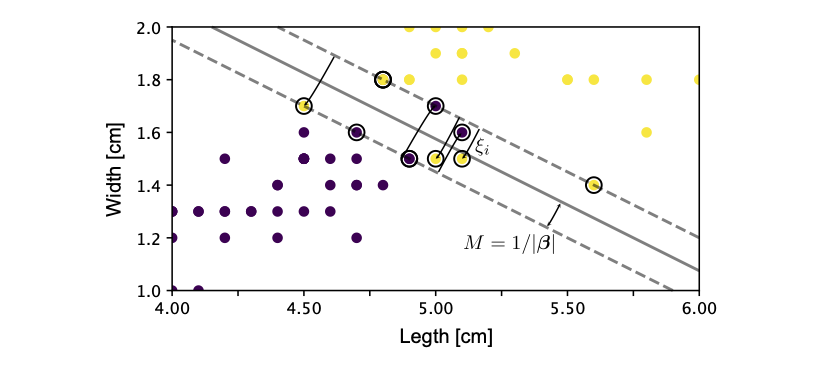
\includegraphics{figures/SVM_overlap}
  \caption{{\bf Binary classification.} Hyperplane separating the two classes and margin $M$ of the linear binary classifier. The support vectors are denoted by a circle around them.}
  \label{fig:svm}
\end{figure}
We can solve this constrained minimization problem by introducing Lagrange multipliers $\alpha_i$ and $\mu_i$ and solving 
\begin{equation}
  \min_{\beta, \{\xi_i\}} \frac12 \sum_{j=1}^{n} \beta_j^2 + C\sum_i \xi_i - \sum_i \alpha_i [y_i \tilde{\bm{x}}_i^T\bm{\beta} - (1-\xi_i)] - \sum_i\mu_i\xi_i,
  \label{eq:svm_lagrange}
\end{equation}
which yields the conditions
\begin{eqnarray}
  \beta_j &=& \sum_i \alpha_i y_i x_{ij},\label{eq:svm_beta}\\
  0 &=& \sum_i \alpha_i y_i\\
  \alpha_i &=& C-\mu_i, \quad \forall i.
\label{eq:svm_derivatives}
\end{eqnarray}
It is numerically simpler to solve the dual problem
\begin{equation}
  \min_{\{\alpha_i\}} \frac12 \sum_{i,i'} \alpha_i \alpha_{i'} y_i y_{i'} \bm{x}_i^T \bm{x}_{i'} - \sum_i \alpha_i
  \label{eq:svm_dual}
\end{equation}
subject to $\sum_i \alpha_i y_i =0$ and $0\leq \alpha_i \leq C$~\footnote{Note that the constraints for the minimization are not equalities, but actually inequalities. A solution thus has to fulfil the additional Karush-Kuhn-Tucker constraints
  \begin{eqnarray}
    \alpha_i [y_i \tilde{\bm{x}}_i^T\bm{\beta} - (1-\xi_i)]&=&0,\label{eq:firstKKT}\\
    \mu_i\xi_i &=& 0,\\
    y_i \tilde{\bm{x}}_i^T\bm{\beta} - (1-\xi_i)&>& 0.
  \end{eqnarray}
}.
Using Eq.~\eqref{eq:svm_beta}, we can reexpress $\beta_j$ to find
\begin{equation}
  f(\bm{x}|\{\alpha_i\}) = \sum_i{}' \alpha_i y_i \bm{x}^T \bm{x}_i + \beta_0,
  \label{eq:svm_f}
\end{equation}
where the sum only runs over the points $\bm{x}_i$, which lie within the margin, as all other points have $\alpha_i\equiv0$ [see Eq.~\eqref{eq:firstKKT}]. These points are thus called the \emph{support vectors} and are denoted in Fig.~\ref{fig:svm} with a circle around them. Finally, note that we can use Eq.~\eqref{eq:firstKKT} again to find $\beta_0$.
\vspace{11pt}

\noindent
\textbf{The Kernel trick and support vector machines}\\
We have seen in our discussion of PCA that most data is not separable linearly. However, we have also seen how the kernel trick can help us in such situations. In particular, we have seen how a non-linear function $\bm{\Phi}(\bm{x})$, which we first apply to the data $\bm{x}$, can help us separate data that is not linearly separable. Importantly, we never actually use the non-linear function $\bm{\Phi}(\bm{x})$, but only the kernel.
Looking at the dual optimization problem Eq.~\eqref{eq:svm_dual} and the resulting classifier Eq.~\eqref{eq:svm_f}, we see that, as in the case of Kernel PCA, only the kernel $K(\bm{x}, \bm{y}) = \bm{\Phi}(\bm{x})^T\bm{\Phi}(\bm{y})$ enters, simplifying the problem. This non-linear extension of the binary classifier is called a \emph{support vector machine}.


\subsubsection{More than two classes: logistic regression}
In the following, we are interested in the case of $p$ classes with $p>2$.
After the previous discussion, it seems natural for the output to take the integer values $y = 1, \dots, p$. However, it turns out to be helpful to use a different, so-called \emph{one-hot encoding}\index{one-hot encoding}. In this encoding, the output $y$ is instead represented by the $p$-dimensional unit vector in $y$ direction $\bm{e}^{(y)}$,
\begin{equation} \label{eqn: One-Hot Encoding}
    y \longrightarrow \bm{e}^{(y)} =
    \begin{bmatrix}
        e^{(y)}_1 \\
        \vdots \\
        e^{(y)}_y \\
        \vdots \\
        e^{(y)}_{p}
    \end{bmatrix}
    =
    \begin{bmatrix}
        0 \\
        \vdots \\
        1 \\
        \vdots \\
        0
    \end{bmatrix},
\end{equation}
where $e^{(y)}_l = 1$ if $l = y$  and zero for all other $l=1,\ldots, p$. A main advantage of this encoding is that we are not forced to choose a potentially biasing ordering of the classes as we would when arranging them along the ray of integers.

A linear approach to this problem then again mirrors the case for linear regression.
We fit a multi-variate linear model, Eq.~\eqref{eqn: Multivariate Linear Model}, to the one-hot encoded dataset \allowbreak$\lbrace(\bm{x}_{1}, \bm{e}^{(y_1)}), \dots, (\bm{x}_{m}, \bm{e}^{(y_m)})\rbrace$. By minimising the RSS, Eq.~\eqref{eqn: RSS}, we obtain the solution
\begin{equation}
    \hat{\beta} = (\widetilde{X}^{T}\widetilde{X})^{-1} \widetilde{X}^{T} Y,
\end{equation}
where $Y$ is the $m$ by $p$ output matrix. The prediction given an input $\bm{x}$ is then a $p$-dimensional vector $\bm{f}(\bm{x}|\hat{\beta}) = \tilde{\bm{x}}^{T} \hat{\beta}$. On a generic input $\bm{x}$, it is obvious that the components of this prediction vector would be real valued, rather than being one of the one-hot basis vectors. To obtain a class prediction $F(\bm{x}|\hat{\beta}) = 1, \dots, p$, we simply take the index of the largest component of that vector, i.e.,
\begin{equation}
    F(\bm{x}|\hat{\beta}) = \textrm{argmax}_{k} f_{k}(\bm{x}|\hat{\beta}).
\end{equation}
The $\textrm{argmax}$ function is a non-linear function and is a first example of what is referred to as \emph{activation function}\index{activation function}. 

For numerical minimization, it is better to use a smooth activation function. Such an activation function is given by the \emph{softmax} function
\begin{equation}
  F_k(\bm{x}|\hat{\beta})= \frac{e^{-f_k(\bm{x}|\hat{\beta})}}{\sum_{k'=1}^pe^{-f_{k'}(\bm{x}|\hat{\beta})}}.
\end{equation}
Importantly, the output of the softmax function is a probability $P(y = k|\bm{x})$, since $\sum_k F_k(\bm{x}|\hat{\beta}) = 1$.
This extended linear model is referred to as \emph{logistic regression}~\footnote{Note that the softmax function for two classes is the logistic function.}.

The current linear approach based on classification of one-hot encoded data generally works poorly when there are more than two classes. We will see in the next chapter that relatively straightforward non-linear extensions of this approach can lead to much better results.
